\begin{comment}

\subsubsection{Some antecedent relationships that imply insufficient antecedent support}

\dots
Let us say that rule~$A$ dominates rule~$B$ if the data captured by~$B$ is a subset of the data captured by~$A$.
%
Rule~$B$ should never follow rule~$A$ in a rule list because it will never capture additional data;
this scenario is a special case where~\eqref{eq:min-capture} immediately applies.
%
More precisely, if~$\RL$ is a rule list that contains rule~$A$ and doesn't contain rule~$B$,
and~$\RL'$ is derived from~$\RL$ by inserting rule~$B$ anywhere after~$A$, then
\begin{align}
\Obj(\RL', \x, \y) = \Obj(\RL, \x, \y) + c \ge \Obj(\RL, \x, \y).
\end{align}
By considering rule semantics, it is easy to think of common situations
leading to dominance relationships between rules.
%
For example, if rule~$A$'s antecedent is~${(x_1 = 0)}$ and rule~$B$'s
antecedent is~${(x_1 = 0) \wedge (x_2 = 1)}$, then rule~$A$ dominates rule~$B$.
%
%Similar to symmetry-aware pruning, we achieve this by restricting how we grow a prefix, as informed by a hash map rdict that maps a rule R_i to a set of rules T_i = {R_k} such that R_i dominates every R_k in T_i. When growing a prefix that ends with rule R_i, we only append a rule R_k if it is not in T_i. Notice that the intersection of S_i and T_i is the empty set, thus the mappings represented by cdict and rdict can easily be combined into a single mapping.
\end{comment}


%Let Q be P's parent. If Q rejects a rule, then P will also reject that rule. This 'inheritance' of rejected rules only depends on which data are captured by Q, and doesn't actually depend on the order of rules in Q. Let S be the set of rules formed from (K-1) rules of P, in any order. P inherits rejected rules from any elements of S. Because of our symmetry-based garbage collection of prefixes equivalent up to a permutation, there are at most K elements of S in the cache; we can identify these via the inverse canonical map (ICM) that maps an ordered prefix to its permutation in the cache. We thus lazily initialize the list of P's reject list of rejected rules.

\begin{comment}

\subsection{Equivalence of rule lists when rules commute}

\begin{theorem}
\end{theorem}

\begin{proof}
\end{proof}

If two rules~$A$ and~$B$ capture disjoint subsets of data,
then they commute globally in the sense that any rule list where~$A$ and~$B$ are
adjacent is equivalent to another rule list where~$A$ and~$B$ swap positions.
%
More generally, a rule list containing possibly multiple, possibly overlapping
pairs of commuting rules is equivalent to any other rule list that can be generated
by swapping one or more such pairs of rules.
%
We can avoid evaluating multiple such equivalent rule lists by eliminating all but one.
%
%We achieve this by restricting how we grow a prefix (by appending a rule), as informed by a hash map cdict that maps each rule R_i to a set of rules S_i = {R_j} such that R_i commutes with every R_j in S_i and j > i. When growing a prefix that ends with rule R_i, we only append a rule R_j if it is not in S_i.

\begin{itemize}
\item other permutation bounds
\end{itemize}
\end{comment}

%For any prefix P, we can write down a lower bound on its permutations' objectives.  (I'm not talking about longer prefixes, just permutations of the same length, call it L.)   An easy bound comes from assuming that there is a permutation that makes no mistakes on captured data, so the only contributions to the objective come from the mistakes of the default rule (call this m) and c*L.  All the permutations capture the same data, so m is constant and this gives

%min objective( any permutation of P ) >= m/n + c*L

%Actually we can make this tighter if we know lower bound information from permutations of sub-prefixes.  For example, the length (L-1) "sub-prefixes" of P generate L permutation groups.  We can add the minimum number of mistakes (on captured data) made by prefixes over all of these groups to our bound, call this k

%min objective( any permutation of P ) >= k/n + m/n + c*L

%We only know k if we've already evaluated the length (L-1) permutations -- we do know it in the breadth-first setting.  (This idea could be generalized to shorter sub-prefixes if desired, e.g., for policies other than breadth first.)

\begin{comment}

\begin{table}[t!]
\centering
\begin{tabular}{l | c | c}
Method & ProPublica & NYCLU \\
\hline
CORELS & 67.6 $\pm$ 2.0 & 69.8 $\pm$ 2.7 \\
SBRL & 67.1 $\pm$ 1.7 & 69.7 $\pm$ 2.0 \\
CART & 66.7 $\pm$ 2.1 & 69.8 $\pm$ 2.7 \\
C4.5 & 67.3 $\pm$ 1.8 & 66.8 $\pm$ 2.1 \\
RF & 67.3 $\pm$ 1.8 & 68.7 $\pm$ 2.4 \\
RIPPER & 67.3 $\pm$ 2.0 & --- \\
AdaBoost & 67.3 $\pm$ 1.7 & 70.6 $\pm$ 2.7 \\
GLM & 67.5 $\pm$ 1.8 & 70.3 $\pm$ 2.5 \\
SVM & 67.1 $\pm$ 2.0 & 70.2 $\pm$ 2.7 \\
\end{tabular}
\vspace{5mm}
\caption{Comparison with other methods:
Means and standard deviations of test accuracy.
Also report algorithm runtimes (mean $\pm$ standard deviation over 10 folds).
CORELS ${\Reg = 0.005}$ for ProPublica and ${\Reg = 0.01}$ for NYCLU.}
\label{tab:comparison}
\end{table}

\begin{figure}[t!]
\begin{center}
\end{center}
\caption{Missing:  Some sort of comparison of different scheduling policies}
\label{fig:scheduling-policy}
\end{figure}

\begin{figure}[t!]
\begin{center}
%\includegraphics[width=0.65\textwidth]{figs/sketch-queue-size.png}
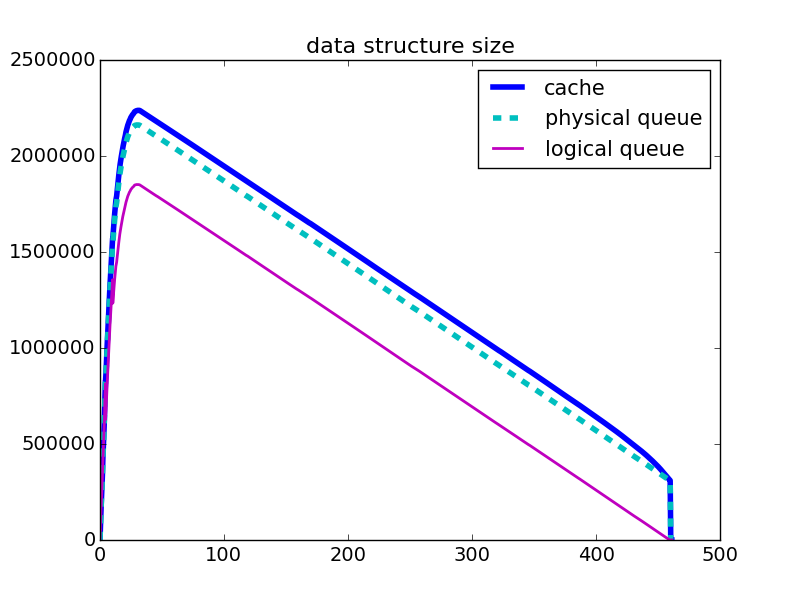
\includegraphics[width=0.8\textwidth]{figs/ela_compas-queue-cache-size-insertions.pdf}
\end{center}
\caption{Cache and queue data structure sizes and insertions.
%
The top plot shows the sizes of the cache and queue data structures,
as a function of wall clock time.
%
The number of nodes in the cache (solid black line) is an
upper bound on the number of elements in the physical queue
(dotted gray line), since the physical queue elements only
correspond to the cache trie data structure's leaf nodes
plus disconnected cache nodes that have been marked for deletion.
%
The queue's physical size is an upper bound on its
logical size (solid blue line), which doesn't include nodes
that have been marked for deletion.
%
The bottom plot shows the cumulative number of cache insertions,
which is equivalent to the cumulative number of queue insertions,
as a function of wall clock time.
}
\label{fig:queue-cache-size-insertions}
\end{figure}

\begin{figure}[t!]
\begin{center}
%\includegraphics[width=0.65\textwidth]{figs/sketch-max-length.png}
\includegraphics[width=0.8\textwidth]{figs/ela-max-length-check.png}
\end{center}
\caption{Max prefix length over time (computed from objective value)}
\label{fig:max-length}
\end{figure}

\begin{figure}[t!]
\begin{center}
\includegraphics[width=0.8\textwidth]{figs/ela_compas-prefix-length.pdf}
\end{center}
\caption{Best prefix length over time}
\label{fig:prefix-length}
\end{figure}
\end{comment}

